\section{Fifth Member}
This is the section dedicated to one of the team members, and it should be written individually . It can include a range of things; first subsection is a space for you to point out the strengths and weaknesses of the module, including complaints about the module coordinator Max Wilson. The second section should have a selfie image with Max! The last part of it is the most important one. You will need to write a paragraph about what you have learned in this module. You can write it in \textbf{Bold} if you want or you can use other fonts. 

Please do not forget:
\begin{itemize}
	\item First paragraph should have your comments about the module
	\item Second one, a selfie img with Max
	\item Last one, what you learned in this module.
\end{itemize}

\subsection{Comments about the module}
Studying software engineering was quite interesting. All the lecture slides were very informative and additional information was available in the extended reading section. Working on the group projects were fun and I learnt a lot through it. The module was well laid out; it was easy to follow through. 
\subsection{Selfie with Max}

To include an image, you will need to remove the comments from the code below, place an image in the main folder, and do not forget to put the name of the image instead of ImgName. 

\begin{figure}[h]
\caption{Max}
\centering
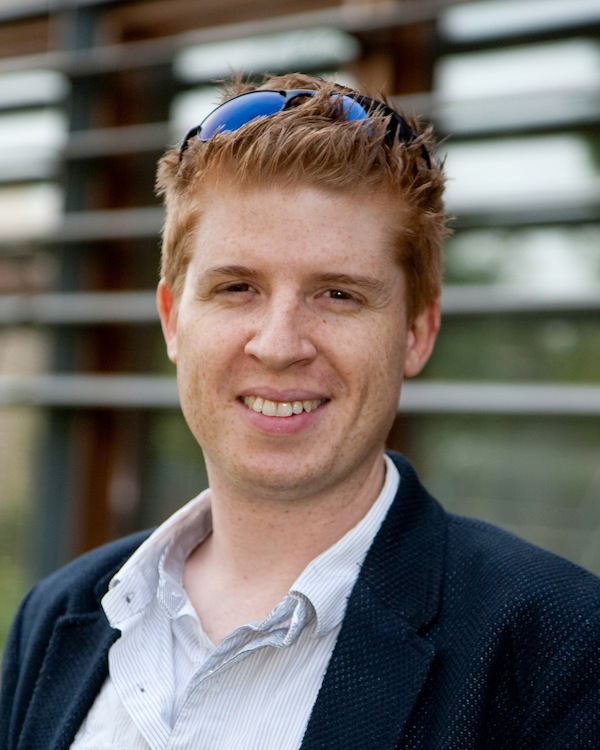
\includegraphics[width=0.5\textwidth]{maxWilson}
\label{fig:selfie}
\end{figure}

You can then use the label of the figure to reference it later with the command ${\backslash}ref$. you can comment out the next line to see an example of how it works.

% My selfie with Max is in  Figure~\ref{fig:selfie}.

\subsection{What I have learned in this module}
In this module, I learnt about the various stages involved in software engineering. First of all, we learnt about Requirements engineering. This involves, how to document the requirements laid by the clients, what the difference between requirements and specifications are etc. We then learnt about prototyping which was very interesting. There are 2 different levels of prototyping; high and low. High is often closer to the finished product and low level prototyping is often created using a paper and pen in the initial stages of prototyping. We then went onto study about testing. Testing is an ongoing process with many stages. Acceptance testing is the final part of the project where  the client agrees that the software works as specified and that the project is over now. Another example of testing is release testing, this is when the project managers decide if it's time to release the project. 

